\chapter{Markov Chain Monte Carlo}
\section{Monte Carlo}
Monte Carlo is a general term for computational techniques that use random
numbers.
Monte Carlo can be used in classical and Bayesian statistics, and a special kind
called Markov Chain Monte Carlo (MCMC) was partially responsible for the revival
of Bayesian statistics in the second half of the 20th century.

What we have seen so far is that you can represent a probability distribution
in a computer by using a vector of possible values and a corresponding
vector of probabilities. For example, suppose we had a single parameter $\theta$
and we had worked out the posterior distribution by using a Bayes' Box. This
will have given us a vector {\tt theta} of possible $\theta$ values and a corresponding
vector {\tt post} containing the posterior probabilities. Well, one thing we could
do is plot the posterior distribution:
\begin{verbatim}
plot(theta, post, xlab="Theta", ylab="Posterior Probability")
\end{verbatim}
This would make a plot something like the following:
\begin{figure}[ht!]
\begin{center}
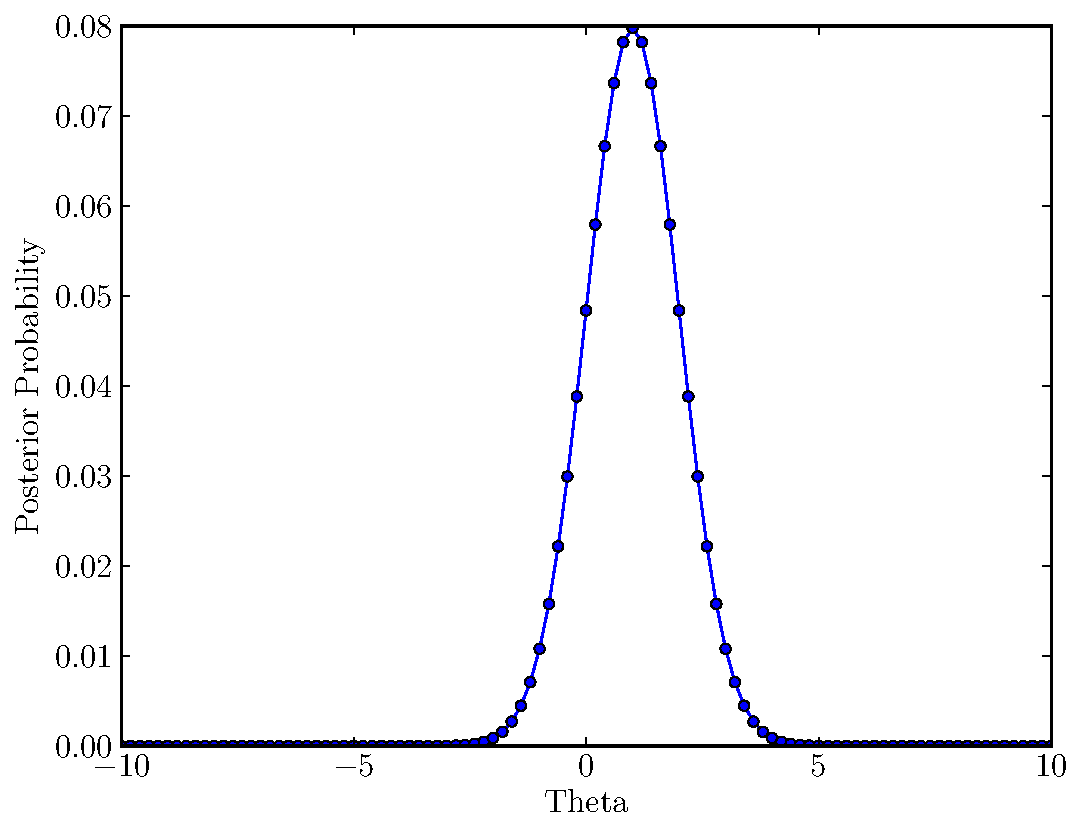
\includegraphics[scale=0.5]{Figures/normal.pdf}
\caption{A posterior distribution can be represented in a computer by a discrete
set of possible parameter values, and the corresponding probabilities.\label{fig:normal}}
\end{center}
\end{figure}
If we wanted to obtain some summaries, we could do it like so:
\begin{verbatim}
post_mean = sum(theta*post)
post_sd = sqrt(sum(theta^2*post) - post_mean^2)
\end{verbatim}

However,
there is an alternative way of representing this posterior distribution in a
computer. It may seem a bit silly at first, because there is nothing wrong with
the above method. But this second method has the advantage that it continues to
work well on much bigger problems, such as when we have more than one parameter.
Instead of having a two vectors: one of $\theta$ values and one of the
corresponding probabilities,
imagine we had some method to compute a random sample of $\theta$ values, drawn
from the posterior distribution. There would only be one vector. So how would we
know that there is greater probability around $\theta=1$? Well, {\it more elements
of the vector would be near 1}. Instead of carrying around a second vector of
probabilities, we simply let the fact that there are lots of points in certain
regions tell us that those regions are more probable! Say our vector of random
samples was called {\tt theta2}. Then we could look at the posterior distribution
by plotting a histogram of samples:
\begin{verbatim}
hist(theta2, breaks=100)
\end{verbatim}
The histogram would look something like this:
\begin{figure}[ht!]
\begin{center}
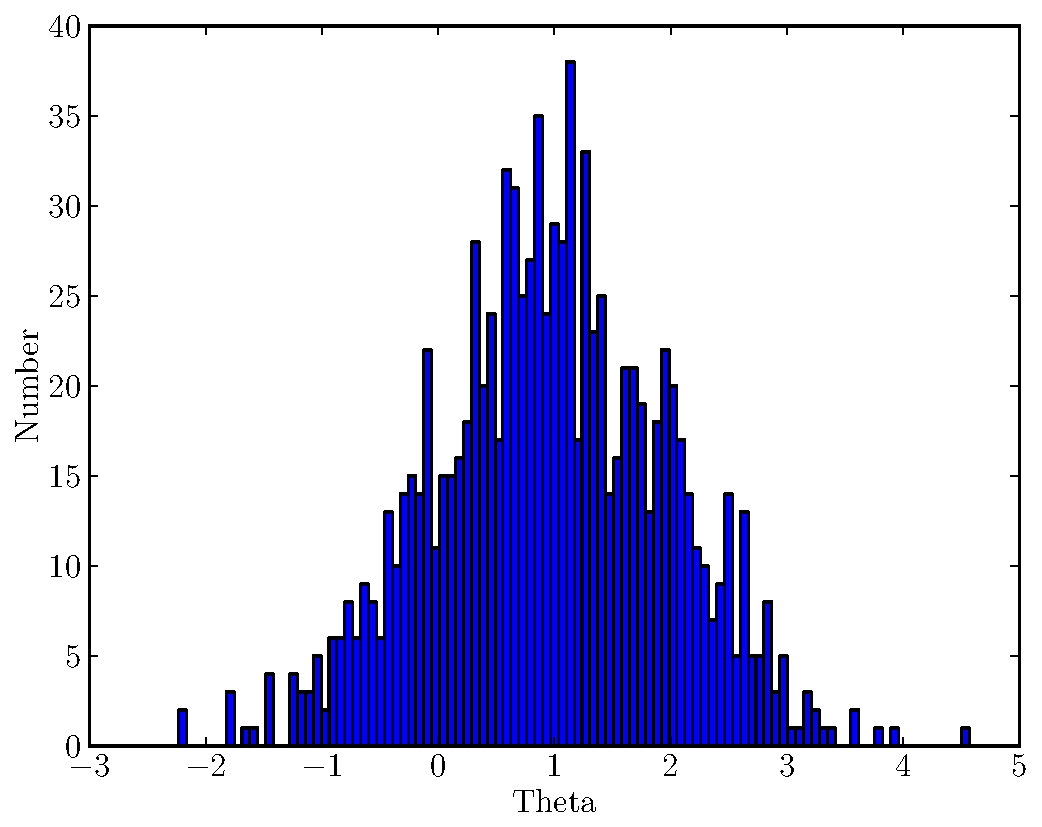
\includegraphics[scale=0.5]{Figures/normal2.pdf}
\caption{The posterior distribution for a parameter $\theta$ can also be
represented by a {\it random sample} of values drawn from the posterior
distribution. The fact that some $\theta$ values are more probable than others
is encoded by the fact that certain values appear more frequently in the sample.
\label{fig:normal2}}
\end{center}
\end{figure}
We could also get our summaries, but the code looks different (It's easier!):
\begin{verbatim}
post_mean = mean(theta2)
post_sd = sd(theta2)
\end{verbatim}
Now, because of the randomness involved in generating the {\tt theta2} samples,
the summaries aren't exact. For example, I know that the actual posterior mean
and standard deviation in this example were both 1, but the values obtained
from the Monte Carlo samples were 0.9604 and 1.0008 respectively. This doesn't
matter much though, because the conclusions about $\theta$ are that it is probably
somewhere around 1 with an uncertainty of about 1, and the error introduced by
using random samples are much smaller than the amount of uncertainty inherent
in the posterior distribution itself.

\begin{framed}
{\bf
The purpose of Markov Chain Monte Carlo is to generate random samples of
parameter values drawn from the posterior distribution. This makes it very easy
to compute summaries even if you have more than one unknown parameter.}
\end{framed}


\section{The Metropolis Algorithm}
The Metropolis algorithm is a fairly simple idea and is the basis of a large
number of MCMC methods. In STATS 331 we will study the basic ideas of what
makes the Metropolis algorithm work. We will look at a small amount of R code
that implements the Metropolis algorithm, but for solving practical problems
it is more convenient to use the JAGS program.

The Metropolis algorithm was invented in the 1940s by physicists, who used it
to do calculations in the field of statistical mechanics. This intriguing field
focuses on calculating the macroscopic (large scale) properties of matter from
knowledge of the small-scale properties: for example, knowing that water is
H$_2$O, you could use statistical mechanics to figure out that if you have a lot
of water molecules, it will freeze at 0 degrees Celsius and boil at 100 degrees
Celsius.

It took
many decades before people started to realise that the Metropolis algorithm was useful in Bayesian
statistics as well. Even though the Bayesian approached seemed very elegant and
useful to many people, it could always be criticised on the basis that, in order
to implement it on practical problems, you usually had to do difficult or
impossible integrals (to summarise the posterior, or to get rid of nuisance
parameters). MCMC changed all that, and is one of the reasons for the
explosion in the popularity of Bayesian statistics beginning in the 1990s.

\begin{framed}
{\bf
The basic idea of MCMC is that we want a method that will travel between
different possible states (such as the possible hypotheses/parameter values in
a Bayesian analysis), and has the property that the amount of time spent in
any particular state is proportional to the posterior probability of that state.}
\end{framed}

\begin{figure}[ht!]
\begin{center}
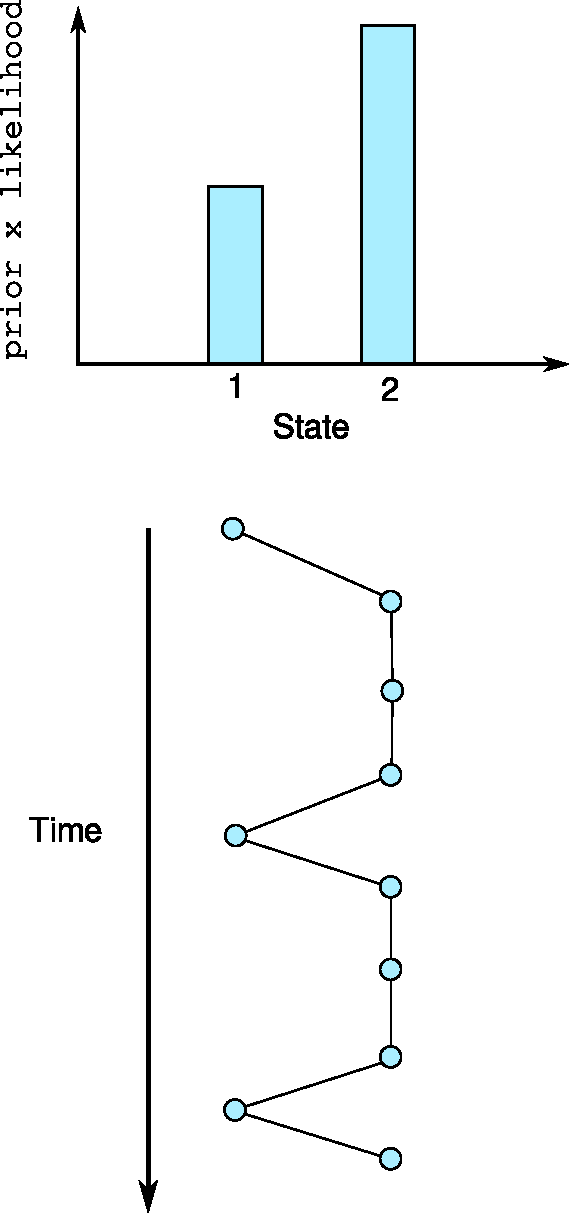
\includegraphics[scale=0.65]{Figures/mcmc.pdf}
\caption{An illustration of the basic idea behind MCMC. Imagine we had a
Bayes' Box with two possible states, and we knew the
{\tt prior $\times$ likelihood} values. The amount of time the MCMC program will
spend in each state is proportional to the posterior probability of the state.
In this example, the MCMC algorithm was in State 1 three times and in State 2
seven times. Using this, we could estimate the posterior probability of State 2
as being 0.7. This estimate would become more accurate if we ran the MCMC for
more iterations.\label{fig:mcmc}}
\end{center}
\end{figure}


\section{Tactile MCMC}

Tactile MCMC is an idea due to Wayne Stewart.
